This section attempts to explain and discuss the key concepts that are the foundation of this project: the POLAR organ persufflation machine and its formal model in VDM; mathematically proving a model in Isabelle and implementing a tool to translate a VDM model into Isabelle HOL; an outline of the problems that this dissertation aims to tackle, as well as the proposed solutions to those problems.

\section{Persufflation}
Organ persufflation is a method for organ preservation in which a donor organ is submerged in a cold preservation solution, a catheter\footnote{A flexible tube inserted through a narrow opening into a body cavity.} is then inserted into the vasculature\footnote{The arrangement of blood vessels in the body, or within an organ.} of the organ and oxygen is pumped into the organ through the catheter, thereby oxygenating\footnote{Supply, treat, charge, or enrich with oxygen.} the organ, see Fig\ref{fig:Persufflation}.\begin{figure}
        \center{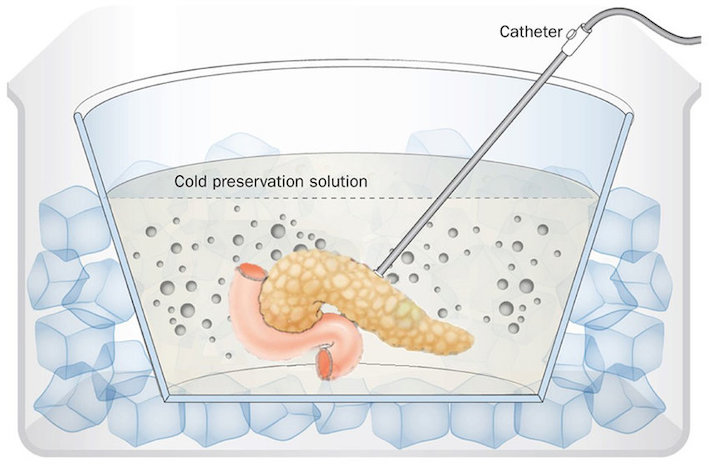
\includegraphics[width=\textwidth]
        {Images/Persufflation.jpeg}}
        \caption{\label{fig:Persufflation} Persufflation \parencite{Dholakia2018}}
      \end{figure} Through this method, more oxygen is delivered to the organ than the other most popular methods and by doing so preservation period can be extended by up to 48-72 hours\parencite{Suszynski2013}. 

However, Persufflation is a delicate process. Oxygen flow, temperature and pressure both inside and outside of the organ must be kept within a precise margin; slightly anomalous variations in any of these variables, could result in damage to the organ. 
Until now, humans have controlled these variables manually: typically, an alarm will sound if a variable exceeds its boundary and an attendant will adjust the value by hand. This method is not precise enough under such safety critical circumstances as human error may result in damage to the organ pre-transplant or failure of the organ post-transplant, due to poor condition.

Through software, the POLAR project's persufflation machine would enable effective, long term persufflation by removing the human element. By exploiting the speed, precision and accuracy of a computer system, POLAR hopes to be able to control these variables with high precision and within a minuscule margin of error. However, as is the nature of software of such complexity, the alarm system that informs changes to variables may be rife with errors, with high potential for unintended behaviour\parencite{JamiaOCW154}. In a safety critical system such as this, it is imperative that software components do not malfunction.


\section{POLAR System Complexity}
The POLAR machine is a Cyber-Physical System - collaborating computational elements controlling physical entities, which interact with humans and their environment. For the sake of keeping safety in mind, it is important to note that the software that will be developed for POLAR is part of a system - a combination of interacting elements organized to achieve one or more stated purposes\parencite{walden_roedler_forsberg_hamelin_shortell_2007}. As such, the system will have several dimensions to take into account - building complexity. Physical variables such as external and internal pressure, temperature, atmospheric composition, movement and more. Also computational variables such as security protocols, fail safes, varying software; Human variables, how will the machine be handled, used, what errors may humans introduce into the system? 

Specifically, human contribution is arguably the central source of error and complexity in a system. Separate discipline-specific development processes result in components being developed in a disjointed manner. In the case of POLAR, software is developed separate to the hardware, a machine engineer is not able to know precisely how their chip's resources will be handled by kernel processes written by the operating system developer, and so they are unable to understand which features might cause error, which limitations the software will have. All of this risks late discovery of defects, namely at the integration stage, when it is highly cumbersome to go back. 

\section{Modelling}
The best way to bridge the gap between varying components, development teams, dimensions of the system, is to create a model of the system, an abstraction of all of these variables together in one unambiguous representation so that the variables of the system can be tested and scrutinised as a whole, their interaction monitored and alterations made where error is found. Models allow us to explore a design space before we build, and physically integrate, the components within it. Interactions are modelled as contracts, assumptions and guarantees of what will or should happen rather than how. As an architect models a structure to smaller scale before it is built - so is a software and hardware system modelled before it is integrated and implemented. This provides evidence for trust, reduces risk of bugs and can even identify improvements to the current design. In POLAR, a system that will someday contribute to human well-being, it is easy to see how an optimal design and faster development will be beneficial. For an increasing amount of software, this model takes the form of a formal specification.

\section{Formal Specification}
Formal specifications are used to describe a system, analyse its behaviour and to aid in its design by verifying key properties of interest through rigorous and effective reasoning tools\parencite{FORMAL1}\parencite{FORMAL2}. These specifications are formal in the sense that they have a syntax, their semantics fall within one domain, and they are able to be used to infer useful information\parencite{Lamsweerde2000}.\parencite{wikiFS} Ordinarily, a formal specification of a system goes no further than a UML diagram of its components and mostly all projects have some form of it. This is a good first approximation, but it is imprecise. For safety critical systems, a mathematical, unambiguous abstraction of the system, which states the effect of computation, is the only acceptable level of specification. A mathematical representation can be analysed, altered and proven using deduction and reasoning techniques - and therefore, so can the design of the system with respect to its specification. A mathematical specification is encoded in an appropriate formal modelling programming language, for POLAR this is VDM-SL.


\section{Vienna Development Method Specification Language (VDM-SL)}
Though readers of this dissertation might already be familiar with VDM, a brief overview of the language is necessary to provide motivation for this project. VDM is a state-based modelling language which allows the modeller to formally specify structure, behaviour and logical constraints. The Vienna Development Method (VDM) was established in the 1970's originating from IBM Laboratory, Vienna. The language has syntax to represent mathematical representation of a specification. Mathematical constructs including, sets, sequences and integers, to name a small few, define types of data that are maintained and transformed in the system. How this data is represented, what restrictions are placed on the data, represented as invariants on types and values, and what data forms the persistent state of the system, define its data set. Behaviour of the system is encoded as functions that represent functionality, and as operations which modify its persistent state. Pre and post conditions for operations and functions are purposeful in both restricting and checking their operation. Errors in the model identify errors in the specification of the system, the specification can then be altered, and the design improved to eliminate errors before the new specification is written in VDM-SL again so that all of this can be repeated. Many iterations of this - model, check, alter, model again - cycle incrementally identify and eliminate errors until none, or as few as possible within a reasonable threshold, can be found.



\subsection{VDM-SL Example, Alarm System}
Below, VDM code represents the alarm system for a nuclear power plant reactor. Experts are paged when certain variables' values cross safe boundaries. Certain experts are on shift at certain times and paging is decided based on period of time over boundaries as well as other important factors such as an expert’s qualification.


\begin{vdmsl}[label=lst:AlarmSL.vdmsl,caption=Types of data used in the alarm system in VDM-SL]
types

Schedule = map Period to set of Expert;

Period = token;

Expert :: expertid : ExpertId
quali : set of Qualification
inv ex == ex.quali <> {};

ExpertId = token;
Qualification = <Elec> | <Mech> | <Bio> | <Chem>;
Alarm :: alarmtext : seq of char
quali : Qualification;
\end{vdmsl}

Above, an invariant on the Expert type is defined to ensure that the expert does not have an empty set of qualifications i.e. the expert is qualified, and their qualifications are recorded.

\begin{vdmsl}[label=lst:AlarmSL.vdmsl,caption=Alarm system's values in VDM-SL]
values
 
  p1:Period = mk_token("Monday day");
  ps : set of Period = {p1,p2,p3,p4,p5};

  eid8:ExpertId = mk_token(190);
  
  e1:Expert = mk_Expert(eid1,{<Elec>});
  exs : set of Expert = {e1,e2,e3,e4,e5,e6,e7,e8};
\end{vdmsl}

Some of the values in the system are shown above. A set of experts is created, one such expert having a particular id and electrical qualification.

\begin{vdmsl}[label=lst:AlarmSL.vdmsl,caption=An alarm system function in VDM-SL which takes a set of experts\, a qualification and returns a boolean value.]
functions
  QualificationOK: set of Expert * Qualification -> bool
  QualificationOK(exs2,reqquali) ==
    exists ex in set exs2 & reqquali in set ex.quali;
\end{vdmsl}
\hfill\break
\hfill\break
\begin{vdmsl}[label=lst:AlarmSL.vdmsl,caption=Alarm system's persistent state in VDM-SL\, t he state is represented as a record type with the important persistent data as fields\, here schedule and alarms.]
state Plant of
schedule : Schedule
alarms : set of Alarm

\end{vdmsl}

\begin{vdmsl}[label=lst:AlarmSL.vdmsl,caption=Operations on the state of the alarm system in VDM-SL\, operations manipulate data stored in the persistent state and mimic the operation of the system.]
operations

NumberOfExperts: Period ==> nat
NumberOfExperts(peri) == is not yet specified
pre peri in set dom schedule;

ExpertIsOnDuty: Expert ==> set of Period

ExpertIsOnDuty(ex) == is not yet specified;

ExpertToPage: Alarm * Period ==> Expert

ExpertToPage(a,peri) == is not yet specified;
\end{vdmsl}

\section{Isabelle Translation}
VDM provides an unambiguous mathematical representation of the system, \textbf{however it does not provide any support for mathematical proof of the specification}. Mathematically proving or disproving correctness of the VDM model and its intended algorithms, allows us to say without doubt that they are correct with respect to their formal specification. Isabelle allows us to write code contracts in Higher Order Logic statements and provides an automated theorem proving assistant to prove them. Code contracts are assumptions and guarantees in the model, features written as VDM constructs. Contracts include but are not limited to: \begin{itemize}
  \item Properties that always hold (i.e. invariants).
  \item Assumptions (pre conditions) and commitments (post conditions).
  \item Proof obligations of interest such as satisfiability\footnote{A logical check to verify that operations are feasible} and reification\footnote{Do representations of the data in the system agree with one another, are they compatible?}, which if proved would establish the consistency of the model.
  \item Proof obligations (POs) of what correctness means, verifying that we have built the correct model.
  \item Sanity checks on functionality, validating that the model has been built correctly.
\end{itemize}
Isabelle is a functional programming language, constructs are represented as fields and curried functions, all collected together in a \syntaxKEYWORDA{theory}, \syntaxKEYWORDA{.thy}, file. A theory is a named collection of types, functions, and theorems, much like a module in a programming language or a specification in a specification language like VDM. Isabelle contains a theory file \syntaxKEYWORDA{"Main"}, which is a union of all the basic, predefined theories like arithmetic, lists, sets, etc. which are used by the automated theorem prover to inform proof assistants. Below, a module \syntaxLITERALA{"VDMToolkit"}\footnote{VDMToolkit is written and maintained by Dr Leonardo Jose Simoes Freitas. Newcastle University.} is included in the imports. This is very important in the VDM to Isabelle translation steps as, similar to \syntaxKEYWORDA{"Main"}, it provides type-checked VDM constructs with pre, post conditions and invariants for VDM types like VDMNat1 and VDMSet, as VDM represents these things differently to Isabelle.

To use Isabelle to prove a model, that model must first be translated from VDM into Isabelle HOL. For the above example, translations are below.

\hfill\break
\hfill\break
\ttfamily
\syntaxNULL{}\gutter{\ \ \ \ 1{|}\ }\syntaxKEYWORDA{theory}{\ }Alarm\hspace*{\fill}\\
\gutter{\ \ \ \ 2{|}\ }\syntaxKEYWORDB{imports}{\ }\syntaxLITERALA{"../../lib/VDMToolkit"}\hspace*{\fill}\\
\gutter{\ \ \ \ 3{|}\ }\syntaxKEYWORDB{begin}\hspace*{\fill}\\
\gutter{\ \ \ 42{|}\ }{\ }{\ }\hspace*{\fill}\\
\gutter{\ \ \ 42{|}\ }{\ }{\ }\hspace*{\fill}\\
\gutter{\ \ \ \ 7{|}\ }\syntaxKEYWORDA{type\usebox{\underscorebox}synonym}{\ }Period{\ }{\ }{\ }\syntaxOPERATOR{=}{\ }VDMToken\hspace*{\fill}\\
\gutter{\ \ \ 14{|}\ }\syntaxKEYWORDA{definition}\hspace*{\fill}\\
\gutterH{\ \ \ 15{|}\ }{\ }{\ }inv\usebox{\underscorebox}Period{\ }\syntaxOPERATOR{::}{\ }\syntaxLITERALA{"Period{\ }⇒{\ }𝔹"}\hspace*{\fill}\\
\gutter{\ \ \ 16{|}\ }{\ }{\ }\syntaxKEYWORDB{where}\hspace*{\fill}\\
\gutter{\ \ \ 17{|}\ }{\ }{\ }\syntaxLITERALA{"inv\usebox{\underscorebox}Period{\ }≡{\ }inv\usebox{\underscorebox}True"}\hspace*{\fill}\\
\gutter{\ \ \ 18{|}\ }{\ }{\ }\hspace*{\fill}\\
\gutter{\ \ \ 19{|}\ }\syntaxKEYWORDA{type\usebox{\underscorebox}synonym}{\ }ExpertId{\ }\syntaxOPERATOR{=}{\ }VDMToken\hspace*{\fill}\\
\gutterH{\ \ \ 20{|}\ }\hspace*{\fill}\\
\gutter{\ \ \ 21{|}\ }\syntaxKEYWORDA{datatype}{\ }Qualification{\ }\syntaxOPERATOR{=}{\ }Elec{\ }\syntaxOPERATOR{|}{\ }Mech{\ }\syntaxOPERATOR{|}{\ }Bio{\ }\syntaxOPERATOR{|}{\ }Chem\hspace*{\fill}\\
\gutter{\ \ \ 22{|}\ }\hspace*{\fill}\\
\gutter{\ \ \ 23{|}\ }\syntaxKEYWORDA{definition}\hspace*{\fill}\\
\gutter{\ \ \ 24{|}\ }{\ }{\ }inv\usebox{\underscorebox}Qualification{\ }\syntaxOPERATOR{::}{\ }\syntaxLITERALA{"Qualification{\ }⇒{\ }𝔹"}\hspace*{\fill}\\
\gutterH{\ \ \ 25{|}\ }{\ }{\ }\syntaxKEYWORDB{where}\hspace*{\fill}\\
\gutter{\ \ \ 26{|}\ }{\ }{\ }\syntaxLITERALA{"inv\usebox{\underscorebox}Qualification{\ }≡{\ }inv\usebox{\underscorebox}True"}\hspace*{\fill}\\
\gutter{\ \ \ 27{|}\ }{\ }{\ }\hspace*{\fill}\\
\gutter{\ \ \ 28{|}\ }\syntaxKEYWORDA{record}{\ }Alarm{\ }\syntaxOPERATOR{=}\hspace*{\fill}\\
\gutter{\ \ \ 29{|}\ }{\ }{\ }alarm\usebox{\underscorebox}alarmtext{\ }\syntaxOPERATOR{::}{\ }\syntaxLITERALA{"char{\ }VDMSeq"}{\ }{\ }\hspace*{\fill}\\
\gutterH{\ \ \ 30{|}\ }{\ }{\ }alarm\usebox{\underscorebox}quali{\ }{\ }{\ }{\ }{\ }\syntaxOPERATOR{::}{\ }Qualification\hspace*{\fill}\\
\gutter{\ \ \ 27{|}\ }{\ }{\ }\hspace*{\fill}\\
\gutter{\ \ \ 38{|}\ }\syntaxKEYWORDA{definition}\hspace*{\fill}\\
\gutter{\ \ \ 39{|}\ }{\ }{\ }inv\usebox{\underscorebox}Alarm{\ }\syntaxOPERATOR{::}{\ }\syntaxLITERALA{"Alarm{\ }⇒{\ }𝔹"}\hspace*{\fill}\\
\gutterH{\ \ \ 40{|}\ }{\ }{\ }\syntaxKEYWORDB{where}\hspace*{\fill}\\
\gutter{\ \ \ 41{|}\ }{\ }{\ }\syntaxLITERALA{"inv\usebox{\underscorebox}Alarm{\ }≡{\ }inv\usebox{\underscorebox}True"}\hspace*{\fill}\\
\gutter{\ \ \ 42{|}\ }{\ }{\ }\hspace*{\fill}\\
\gutter{\ \ \ 43{|}\ }\syntaxKEYWORDA{record}{\ }Expert{\ }\syntaxOPERATOR{=}\hspace*{\fill}\\
\gutter{\ \ \ 44{|}\ }{\ }{\ }expert\usebox{\underscorebox}expertid{\ }{\ }\syntaxOPERATOR{::}{\ }ExpertId\hspace*{\fill}\\
\gutterH{\ \ \ 45{|}\ }{\ }{\ }expert\usebox{\underscorebox}quali{\ }{\ }{\ }{\ }{\ }\syntaxOPERATOR{::}{\ }\syntaxLITERALA{"Qualification{\ }VDMSet"}\hspace*{\fill}\\
\gutter{\ \ \ 46{|}\ }{\ }{\ }\hspace*{\fill}\\
\gutter{\ \ \ 47{|}\ }\syntaxKEYWORDA{definition}\hspace*{\fill}\\
\gutter{\ \ \ 48{|}\ }{\ }{\ }inv\usebox{\underscorebox}Expert{\ }\syntaxOPERATOR{::}{\ }\syntaxLITERALA{"Expert{\ }⇒{\ }𝔹"}\hspace*{\fill}\\
\gutter{\ \ \ 49{|}\ }{\ }{\ }\syntaxKEYWORDB{where}\hspace*{\fill}\\
\gutterH{\ \ \ 50{|}\ }{\ }{\ }\syntaxLITERALA{"inv\usebox{\underscorebox}Expert{\ }e{\ }≡}\hspace*{\fill}\\
\gutter{\ \ \ 51{|}\ }\syntaxLITERALA{{\ }{\ }{\ }{\ }{\ }{\ }let{\ }eq{\ }={\ }(expert\usebox{\underscorebox}quali{\ }e){\ }in{\ }}\hspace*{\fill}\\
\gutter{\ \ \ 52{|}\ }\syntaxLITERALA{{\ }{\ }{\ }{\ }{\ }{\ }{\ }{\ }inv\usebox{\underscorebox}SetElems{\ }inv\usebox{\underscorebox}True{\ }eq{\ }∧}\hspace*{\fill}\\
\gutter{\ \ \ 53{|}\ }\syntaxLITERALA{{\ }{\ }{\ }{\ }{\ }{\ }{\ }{\ }eq{\ }≠{\ }\usebox{\opencurlybracket}\usebox{\closecurlybracket}"}\hspace*{\fill}\\
\gutter{\ \ \ 54{|}\ }\hspace*{\fill}\\
\gutter{\ \ \ 74{|}\ }\syntaxKEYWORDA{type\usebox{\underscorebox}synonym}{\ }Schedule{\ }\syntaxOPERATOR{=}{\ }\syntaxLITERALA{"Period{\ }⇀{\ }Expert{\ }set"}{\ }\hspace*{\fill}\\
\gutterH{\ \ \ 75{|}\ }{\ }{\ }\hspace*{\fill}\\
\gutter{\ \ \ 77{|}\ }\syntaxKEYWORDA{definition}\hspace*{\fill}\\
\gutter{\ \ \ 78{|}\ }{\ }{\ }inv\usebox{\underscorebox}Schedule{\ }\syntaxOPERATOR{::}{\ }\syntaxLITERALA{"Schedule{\ }⇒{\ }𝔹"}\hspace*{\fill}\\
\gutter{\ \ \ 79{|}\ }{\ }{\ }\syntaxKEYWORDB{where}\hspace*{\fill}\\
\gutterH{\ \ \ 80{|}\ }{\ }{\ }\syntaxLITERALA{"inv\usebox{\underscorebox}Schedule{\ }s{\ }≡{\ }}\hspace*{\fill}\\
\gutter{\ \ \ 81{|}\ }\syntaxLITERALA{{\ }{\ }{\ }{\ }{\ }{\ }inv\usebox{\underscorebox}Map{\ }inv\usebox{\underscorebox}Period{\ }(inv\usebox{\underscorebox}SetElems{\ }inv\usebox{\underscorebox}Expert){\ }s{\ }}\hspace*{\fill}\\
\gutter{\ \ \ 82{|}\ }\syntaxLITERALA{{\ }∧}\hspace*{\fill}\\
\gutter{\ \ \ 83{|}\ }\syntaxLITERALA{{\ }{\ }{\ }{\ }{\ }{\ }(∀{\ }exs1{\ }∈{\ }rng{\ }s{\ }.{\ }}\hspace*{\fill}\\
\gutter{\ \ \ 84{|}\ }\syntaxLITERALA{{\ }{\ }{\ }{\ }{\ }{\ }{\ }{\ }{\ }{\ }exs1{\ }≠{\ }\usebox{\opencurlybracket}\usebox{\closecurlybracket}{\ }∧}\hspace*{\fill}\\
\gutterH{\ \ \ 85{|}\ }\syntaxLITERALA{{\ }{\ }{\ }{\ }{\ }{\ }{\ }{\ }{\ }{\ }(∀{\ }ex1{\ }∈{\ }exs1{\ }.{\ }∀{\ }ex2{\ }∈{\ }exs1{\ }.{\ }}\hspace*{\fill}\\
\gutter{\ \ \ 86{|}\ }\syntaxLITERALA{{\ }{\ }{\ }{\ }{\ }{\ }{\ }{\ }{\ }{\ }{\ }{\ }{\ }{\ }ex1{\ }≠{\ }ex2{\ }⟶{\ }(expert\usebox{\underscorebox}quali{\ }ex1){\ }≠{\ }(expert\usebox{\underscorebox}quali{\ }ex2)))"}\hspace*{\fill}\\
\gutter{\ \ \ 87{|}\ }{\ }{\ }\hspace*{\fill}\\
\gutter{\ \ 716{|}\ }\syntaxKEYWORDB{end}\hspace*{\fill}\\
\hfill\break
\hfill\break
\rmfamily
The translation 'recipe' detailing the general method for translation will be detailed in the Implementation section of this document later, see \ref{itr}. It is evident that translations might become very intricate and cumbersome for more complex models, human error during repetitive tasks is common, and manual translation takes time. The complexity comes from the level of detail required for each VDM construct's translation: each type must have an invariant checking all of its subsequent types; when it comes to function translations, which we will see later, each function needs a pre and a post condition also; state must be initialised in a separate function which must also have a pre and a post condition and so on. The tool, whose development is detailed in the next chapter, automates translation to leave the modeller free to concentrate on proving the translated model rather than translating it manually - and consequently spending time fixing minor errors and filling in gaps in that translation. \footnote{See the Isabelle manual for more information: https://isabelle.in.tum.de/dist/Isabelle2018/doc/tutorial.pdf}